% -*- root: ../../main.tex -*-
Paxos è un algoritmo di consenso, non resistente a Byzantine Fault, sviluppato verso la fine degli anni ottanta e pubblicato nel 1998. Esso ha ricoperto il ruolo di algoritmo standard per decenni, venendo utilizzato in diversi ambienti, compreso quello didattico, poichè rappresenta un'ottima alternativa al commit a due fasi e a quello a tre fasi che si affidano entrambi ad un unico coordinatore che rappresenta un single point of failure. Esistono molte varianti di Paxos, ma la più usata si chiama \textit{Single Decree Paxos}.

In Paxos, i nodi possono assumere contemporaneamente uno o più dei seguenti ruoli:
\begin{itemize}
	\item \textbf{Proposer:} propone un valore su cui accordarsi a tutti gli acceptor.
	\item \textbf{Acceptor:} riceve le proposte dei proposer, decide se accettarle o meno e inoltra la propria risposta ai learner.
	\item \textbf{Learner:} sulla base delle risposte ricevute, determina come valore vincitore quello scelto dalla maggioranza degli acceptor.
\end{itemize}


  \begin{figure}[H]
    \centering
    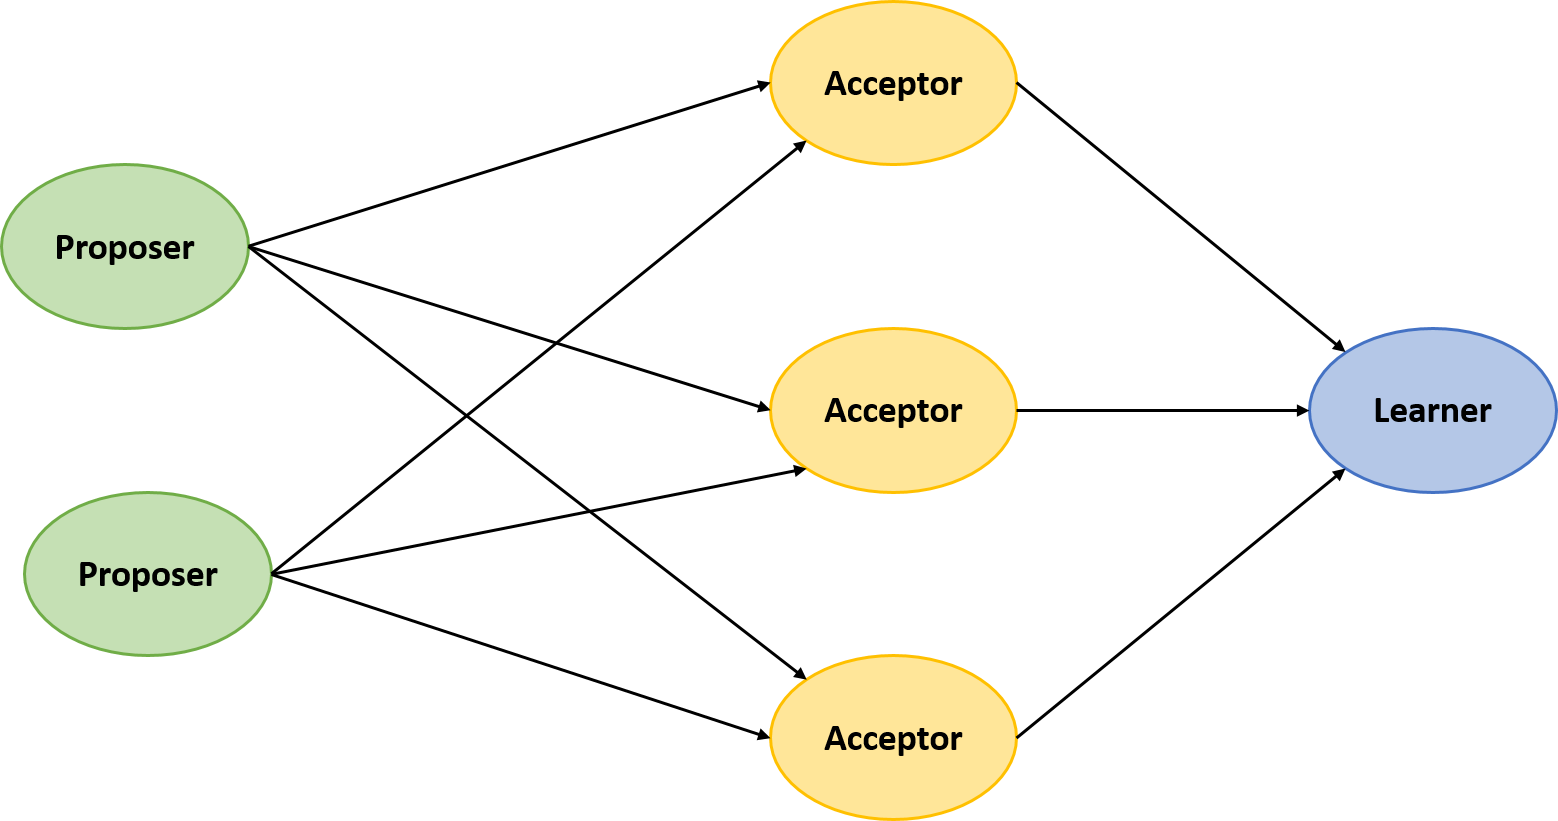
\includegraphics[width=0.90\columnwidth]{paxos/proposeAcceptLearn.png}
    \caption{Esempio di configurazione dei ruoli con due \textbf{proposer}, tre \textbf{acceptor} e un \textbf{learner} che sono rappresentati come nodi distinti per semplicità: nella realtà un nodo può ricoprire più di un ruolo alla volta.}
    \label{fig:figure 5}
  \end{figure}


Qualsiasi criterio si scelga per far decidere agli acceptor quale valore accettare, si incorre in casi di \textbf{incorrettezza} a meno di non utilizzare un approccio in due passi. 
Il raggiungimento del consenso si sviluppa quindi in due fasi.

\begin{enumerate}
	\item \textbf{Proposal:} in questa fase i proposer inviano una richiesta di \textbf{\textit{prepare(n)}} agli acceptor, dove \textit{n} è un \textit{proposal number} scelto in maniera tale che sia maggiore di ogni altro numero incontrato fino a quel momento.\\
  Gli acceptor ricevono le proposte e, per ognuna, controllano se il valore corrispondente è il maggiore in cui si siano imbattuti fino a quel momento: in caso affermativo, rispondono alla proposta impegnandosi a non accettare proposte precedenti, altrimenti la ignorano.\\
  Se un proposer riceve una risposta alla propria proposta dalla maggiorparte degli acceptor, passa alla seconda fase.
	
	\item \textbf{Accept:} in questa fase, il proposer invia il \textbf{proposal number} e il \textit{value} tramite una richiesta \textbf{\textit{accept(n,v)}} rivolta a tutti gli acceptor.\\
  Se il proposer si vede ritornare come risposta il proprio \textit{proposal number} valore, allora la maggioranza degli acceptor ha concordato sul valore proposto, che quindi sarà quello scelto.\\
  Nel caso in cui ciò non accada, il proposer si vedrà arrivare un \textit{proposal number} maggiore del poprio, di conseguenza ricomincerà l'iter, tornando all'inizio della prima fase.
\end{enumerate}

  \begin{figure}[H]
    \centering
    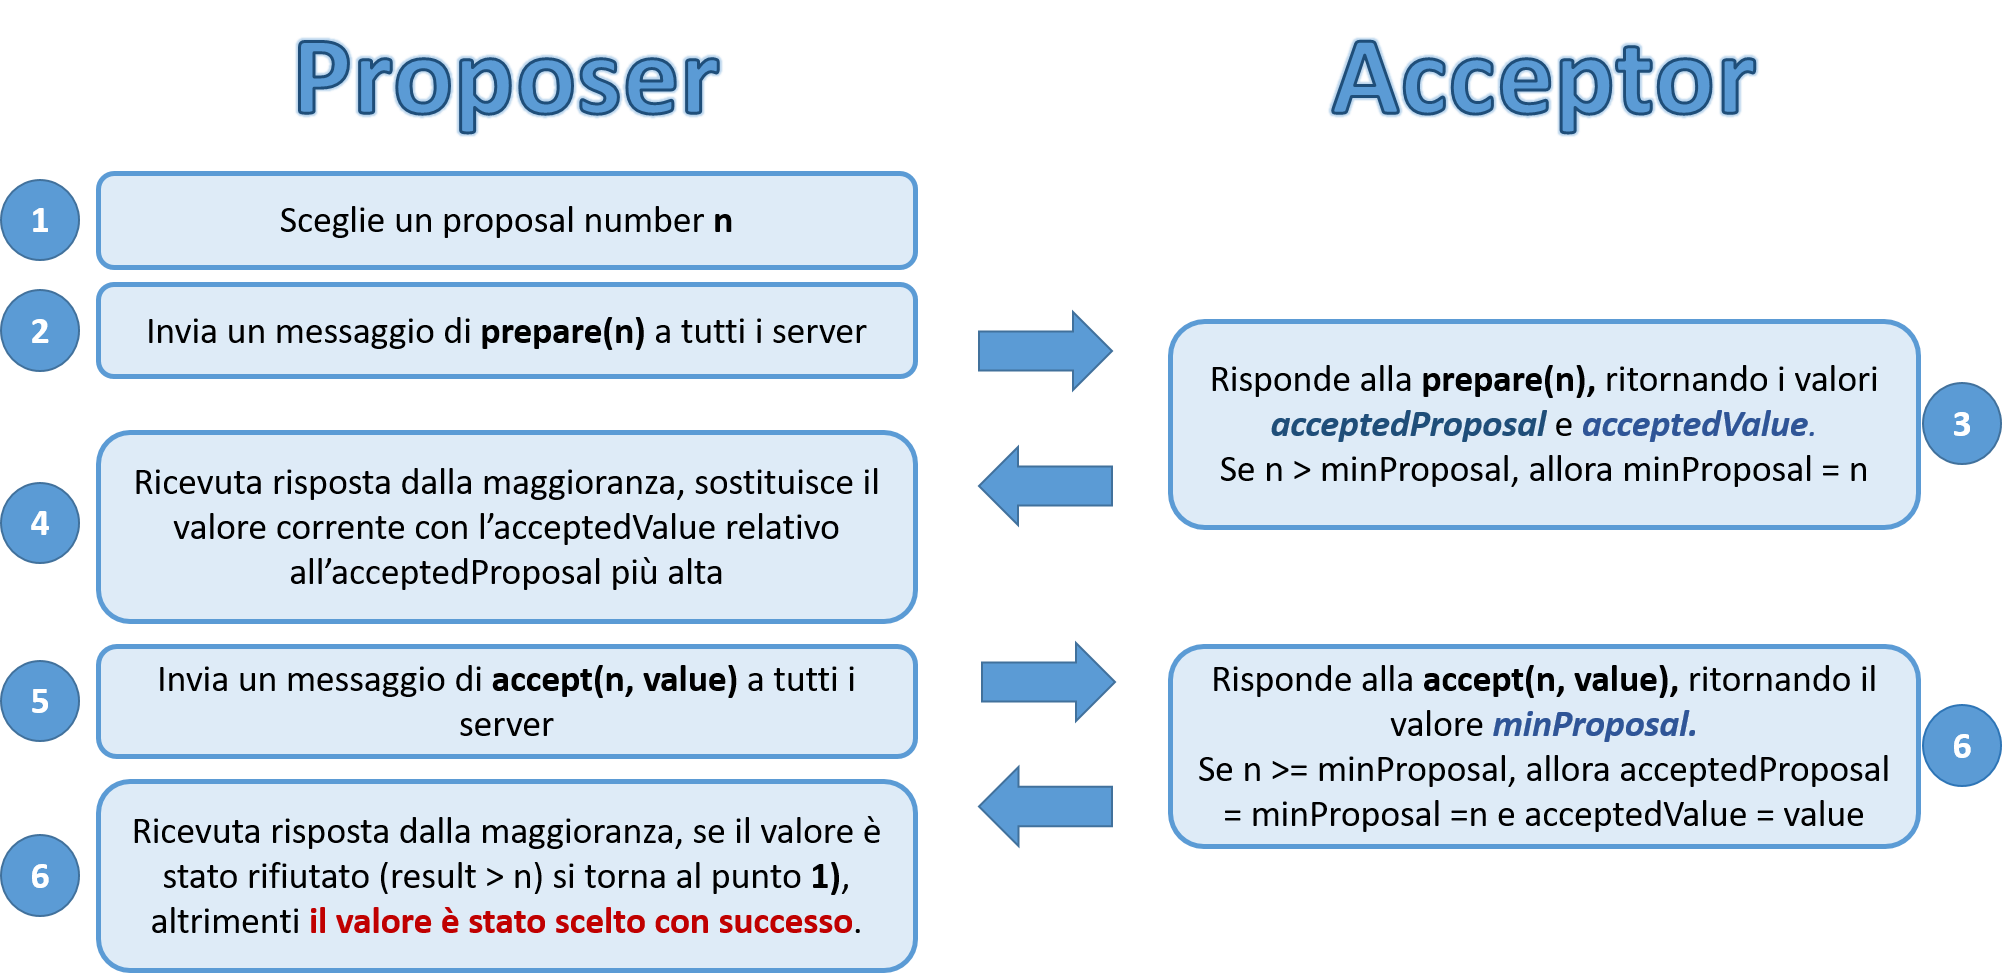
\includegraphics[width=0.90\columnwidth]{paxos/proposersAcceptorsInteraction.png}
    \caption{Schema riassuntivo delle interazioni tra proposer e acceptor, che non tiene conto, per semplicità, dei learner}
    \label{fig:figure 6}
  \end{figure}

L'algoritmo Paxos non è così semplice come potrebbe sembrare a una prima lettura, ma nasconde una serie di dinamiche complesse che non verranno analizzate in questo elaborato poichè è sufficiente un'infarinatura sul funzionamento generale di Paxos per capire in cosa differisce RAFT. 

\subsection{Problemi di Paxos}
  Nonostante sia ancora largamente usato, l'algoritmo Paxos presenta dei difetti che RAFT ha provato a colmare:
  \begin{itemize}
  	\item \textbf{Difficoltà di comprensione:} la parte teorica e le dinamiche dell'algoritmo sono di difficile comprensione e spiegazione, come evidenziato anche dagli esperimenti condotti dagli autori di RAFT.
  	
  	\item \textbf{Difficoltà di implementazione:} anche una volta assimilata la parte teorica, è difficile applicarla. Quando si scende nei dettagli implementativi si va in contro a una confusione generale data dalla presenza di diverse interpretazioni, spesso errate.

  	\item \textbf{Inefficienza:} prima che ci si possa accordare su un valore sono necessari almeno due round.

  	\item \textbf{Valore unico:} il consenso viene raggiunto su un unico valore, per tutta la durata vitale del sistema.

  	\item \textbf{Convergenza:} non è garantito che l'algoritmo converga, arrivando a una soluzione. L'unica garanzia è che se converge, il valore scelto sarà uno e uno solo.
  \end{itemize}